% !TEX root = ../../../main.tex

\begin{figure}[!htbp]
    \centering
    \begin{subfigure}[b]{0.07\textwidth}
        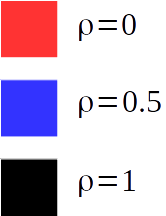
\includegraphics[width=\textwidth]{colorbar/rho.png}
        \vspace{0.2in}
    \end{subfigure}
    \begin{subfigure}[b]{0.35\textwidth}
        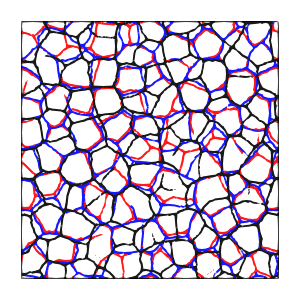
\includegraphics[width=0.6\textwidth]{past/figures/psic_constant.png}
    \end{subfigure}
    \begin{subfigure}[b]{0.07\textwidth}
        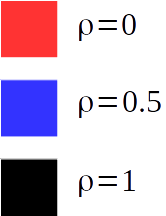
\includegraphics[width=\textwidth]{colorbar/rho.png}
        \vspace{0.2in}
    \end{subfigure}
    \begin{subfigure}[b]{0.35\textwidth}
        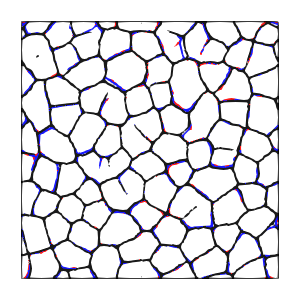
\includegraphics[width=0.6\textwidth]{past/figures/Gc_constant.png}
    \end{subfigure}
    
    \begin{subfigure}[b]{0.25\textwidth}
        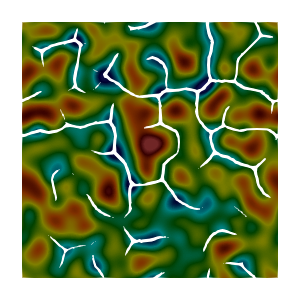
\includegraphics[width=0.7\textwidth]{past/figures/Gc_sqexp_cartesian_5_5_rho_0_seed_a_with_crack_140.png}
    \end{subfigure}
    \begin{subfigure}[b]{0.25\textwidth}
        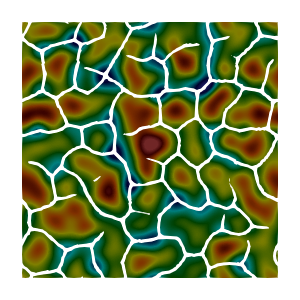
\includegraphics[width=0.7\textwidth]{past/figures/Gc_sqexp_cartesian_5_5_rho_0_seed_a_with_crack_160.png}
    \end{subfigure}
    \begin{subfigure}[b]{0.25\textwidth}
        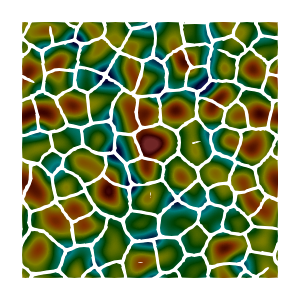
\includegraphics[width=0.7\textwidth]{past/figures/Gc_sqexp_cartesian_5_5_rho_0_seed_a_with_crack_220.png}
    \end{subfigure}
    \begin{subfigure}[b]{0.05\textwidth}
        \caption*{$\Gc^*$}
        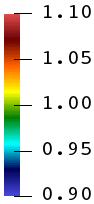
\includegraphics[width=\textwidth]{colorbar/rainbow_vertical.png}
    \end{subfigure}

    \begin{subfigure}[b]{0.25\textwidth}
        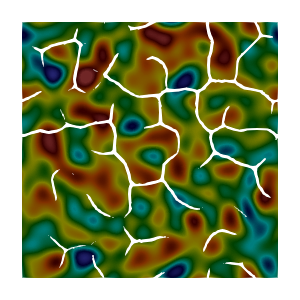
\includegraphics[width=0.7\textwidth]{past/figures/psic_sqexp_cartesian_5_5_rho_0_seed_a_with_crack_140.png}
    \end{subfigure}
    \begin{subfigure}[b]{0.25\textwidth}
        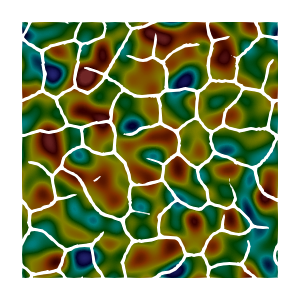
\includegraphics[width=0.7\textwidth]{past/figures/psic_sqexp_cartesian_5_5_rho_0_seed_a_with_crack_160.png}
    \end{subfigure}
    \begin{subfigure}[b]{0.25\textwidth}
        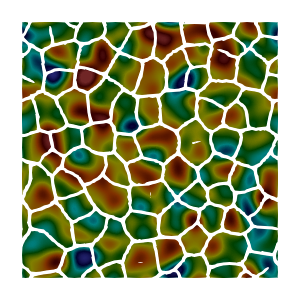
\includegraphics[width=0.7\textwidth]{past/figures/psic_sqexp_cartesian_5_5_rho_0_seed_a_with_crack_220.png}
    \end{subfigure}
    \begin{subfigure}[b]{0.05\textwidth}
        \caption*{$\pi_c^*$}
        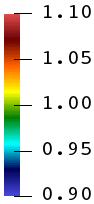
\includegraphics[width=\textwidth]{colorbar/rainbow_vertical.png}
    \end{subfigure}
\end{figure}
